\subsection{Agent network conceptualization}
\label{Agent_newtork_conceptualization}
In the following section we will describe the system in a general way using sensors and not cameras. Furthermore the network always try to optimize those two criterion:
\begin{itemize}
    \item Reduce as much as possible the need for communications.
    \item Algorithm with a low complexity because we consider a small computational power.
\end{itemize}

In such a system most of the communication processes complexity grows in $O^n$. When considering less then five agent it does not matter but if there are hundred of them it can become a problem. Therefore it seems important to reduce as much as possible the communication. 

\subsubsection{Network main structure}
A network is a structure composed by multiple agent. The definition of agent varies slightly and every one does not agree  the same definition so let's clarify it before going futher. In the system, the agent are defined as followed : 
    
\begin{itemize}
    \item Autonomous :  
    \item Sociable :
    \item Reactive :
    \item Pro-active :
\end{itemize}
 
\begin{wrapfigure}{r}{10cm}
    \centering
    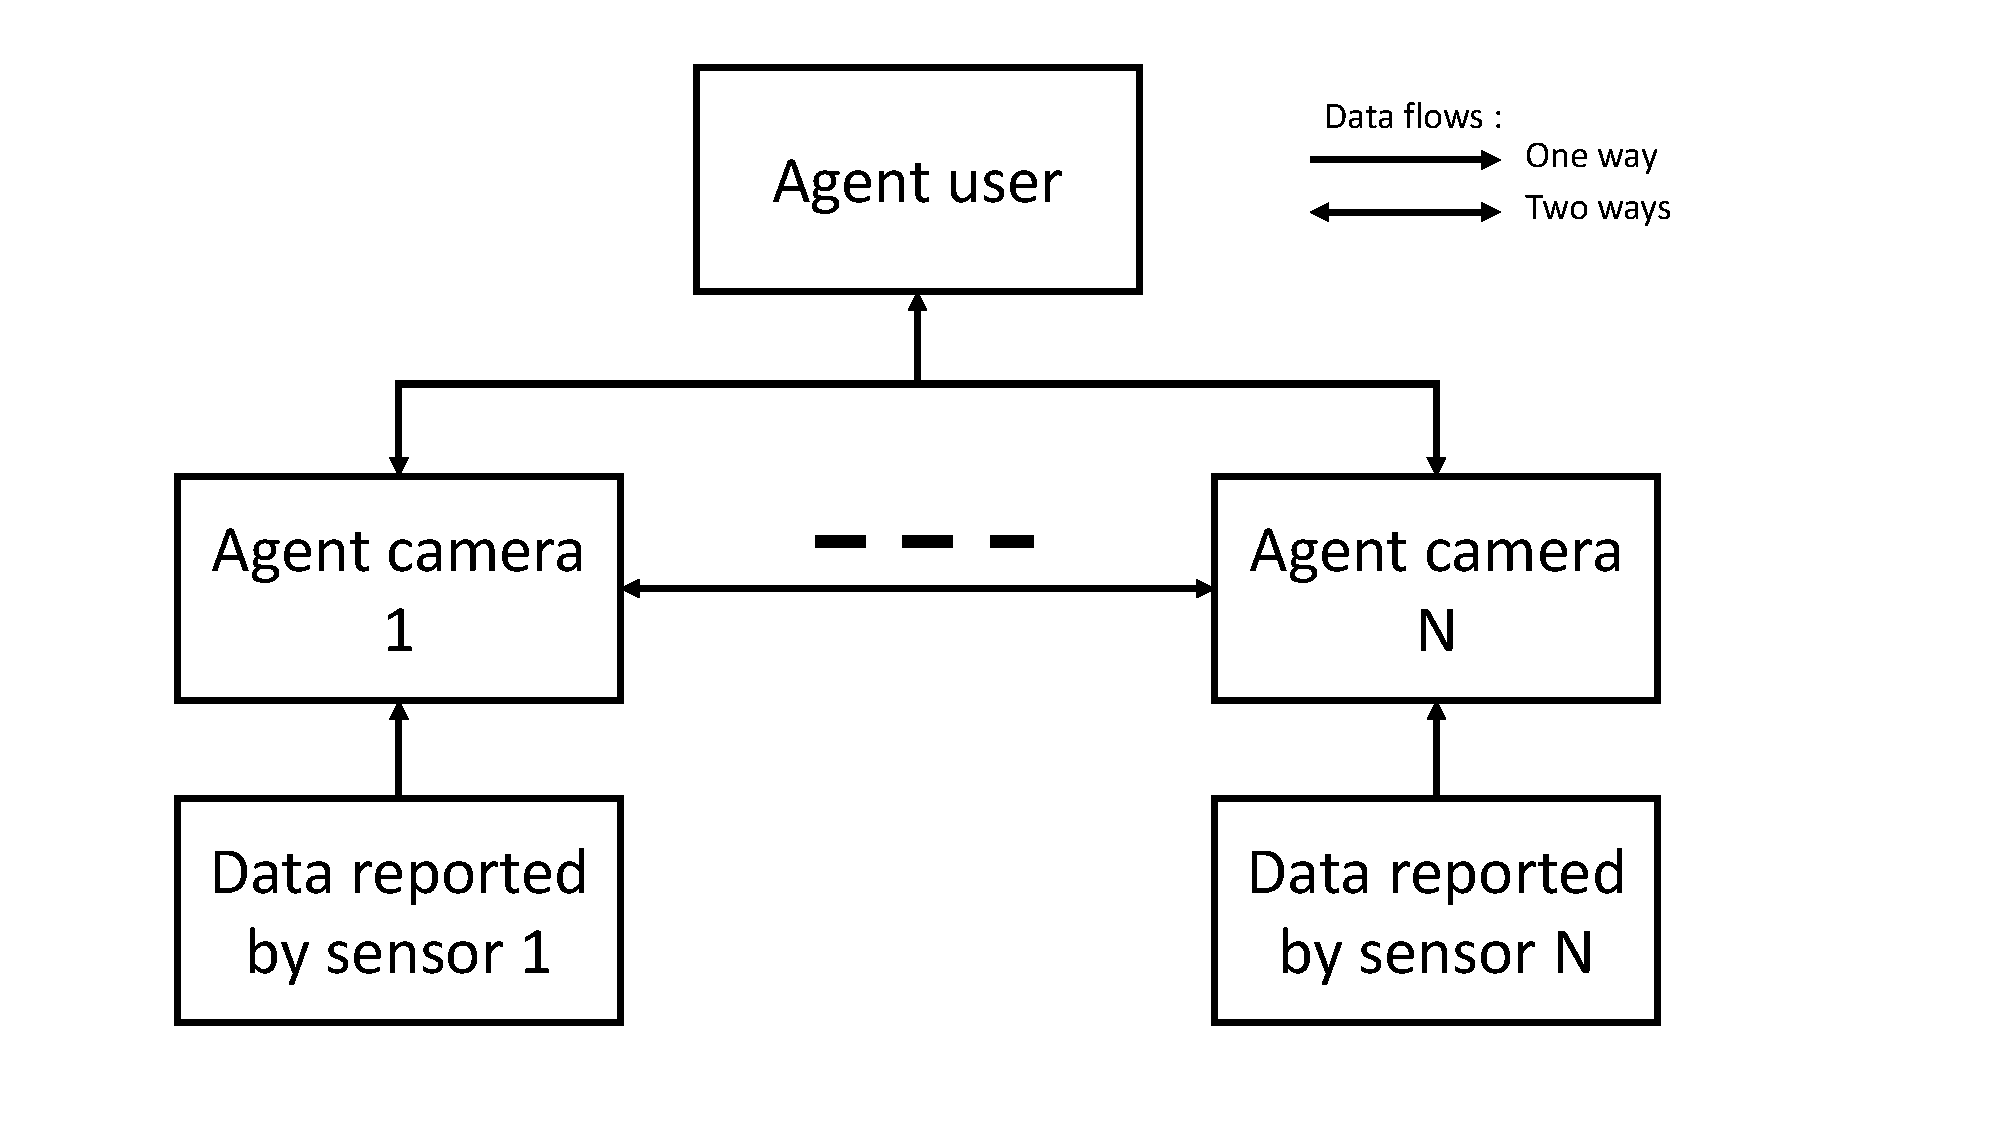
\includegraphics[page=1,clip,width = 8cm]{systeme_multi_agent/conceptualization/multi_agent_schematic.pdf}
    \caption{Global network overview}
    \label{fig:Network_overview}
\end{wrapfigure}


As shown in the figure \ref{fig:Network_overview} the network is rather simple and composed by two type of agents. Arrows in the bloc diagram represent how information flows. Data are given to the first layer that is a set of \notreVocabulaire{agent sensors}. This layer acts as a filter and transmits the relevant information from the data to the second layer which is called \notreVocabulaire{agent user} and is the output.\\

It is also important to point out that agents are equals from a hierarchical point of view and can communicate together at anytime. Their specific role is clarified in the following sections.



\subsubsection{Agent user}
The \notreVocabulaire{agent user} clusters \notreVocabulaire{agents sensors}. It collects data coming from multiple sources and operates a fusion to summarize the essential content to the user . It plays a passive role because it cannot give orders to an other agent.\\

The fusion process is possible because each information received about a target contains a timestamp and a confidence coefficient. When multiple data are received for the same target, the \notreVocabulaire{agent user} compares information and keeps the more recent one with the higher confidence. 


\subsubsection{Agent sensors}
The \notreVocabulaire{agent sensors} is the principal piece in the network. Its role is to analyse the data given by a sensor (in this case a camera) and to cooperate with the other \notreVocabulaire{agents sensors} to compare similarities in data gathered. This cooperation aims mainly to reduce noise and avoid obstructions. It also helps to take a decision to set senors in a suitable configuration, if they can move.\\

The starting point of the agent nature is the first criteria stated at the top of section \ref{Agent_newtork_conceptualization}, the goal is to reduced the communication not to overload the system when to many agents are used.First of all the agent create a virtual situation based on information collected in the real situation. The information is either obtained thanks to a sensor or by communication means. Each agent has thereby its own belief of the real situation and uses it to take decision. The second point is that each algorithm is linear, then when two agents have the same beliefs they will act in the same way.\\

\begin{wrapfigure}{r}{10cm}
    \centering
    \includegraphics[page=2,clip,width = 10cm]{systeme_multi_agent/conceptualization/multi_agent_schematic.pdf}
    \caption{Description of belief}
    \label{fig:Belief_description}
\end{wrapfigure}

Assuming now that agents have always the same believes  then they can coordinate themselves without communicating. They are able to predict how they would act if they were in the situation of the other agents thus communication is no more required. This  hypothesis is to strong, in practice believes diverges and communication is partially use to synchronise them.\\


The figure \ref{fig:Belief_description} illustrate how the above principle works. The belief is the one from agent 3. Part of the information comes from the sensors and the rest is sent by the other agents. In this case agent 5 will send an information about target 5 to agent 3. This information is added between the old and the new belief. One can also notice that agent 4 is not represented in the belief. This represent a situation where agent 4 is inactive and thus agent 3 cannot anticipate what it is doing. This small example already shows how hard it is to keep all the believes synchronised.\\

Based on this beliefs the agent is the able to act. This behaviour is described in the section \ref{agent_camera_implementation} because it is specific to the given use case described in section \ref{Use_case}.






\subsubsection{Communications processes}
The communication is in the center of the hole system. Isolated, an agent is useless and it needs to share information in order to become powerful. Agents communicate together with a defined code. This section will explain the different type of messages and their role in the all system. The figure \ref{fig:communication_flows} summarizes the different messages and how agents exchange them.\\

\begin{figure}[h!]
    \centering
    \includegraphics[page=3,clip,width = 8cm]{systeme_multi_agent/conceptualization/multi_agent_schematic.pdf}
    \caption{Communication flows between agent}
    \label{fig:communication_flows}
\end{figure}

\notreVocabulaire{Heartbeats} messages are the simplest one but rather essential. In the schematic they are shown by the yellow arrows. In fact there is no exchange of information about targets or agents however it allows modularity in the system. At the start each agent considers all the other as inactive but as soon as it receives \notreVocabulaire{Heartbeats}, they will start to operate together. Now let's imagine an agent stops suddenly working well and therefore stop sending messages, then it will be set back as inactive by the others. The problem is though detected and the remaining agents can try to compensate this loss. Nevertheless as soon as it recovers and sends \notreVocabulaire{Heatbeats} again, then the others will set it back to active and the situation is restored to the point before the problem happends.\\

\notreVocabulaire{Related targets information} are use in every cases. The main goal is to share data either to synchronise the believes or to bring redundancy to be able to filter the data.\\

\notreVocabulaire{Related agents information} are used only when sensors can move in space. It creates a need to update the believes about other agent configuration because it can varies with respect to time. 

